% \listfiles
\documentclass[usenames,dvipsnames]{beamer}
\mode<presentation>
\usecolortheme{crane}

\hfuzz=40pt
\setbeamertemplate{navigation symbols}{
    \usebeamerfont{footline}
    \usebeamercolor[fg]{footline}
    \hspace{1em}
    \insertframenumber/\inserttotalframenumber
}

\setbeamertemplate{caption}{\raggedright\insertcaption\par}
% \setbeamercovered{dynamic}
\setbeamercovered{still covered={\opaqueness<1->{15}},again covered={\opaqueness<1->{70}}}
\input{libs}
% Commands
\newcommand{\edge}[3][]{
	\draw[#1] (#2) edge (#3);
}

\newcommand{\edgeWithLabel}[4][]{
	\draw[#1] (#2) edge node[edge label]{#3} (#4);
}

\newcommand{\twocolors}[1]{
	\fill[fill=orange] (#1.west) -- (#1.east) arc(0:180:7.5pt);
	\fill[fill=blue] (#1.west) -- (#1.east) arc(0:-180:7.5pt);
	\node at(#1){};
}

%  Nodes
\tikzset{
	,c1/.style={fill=green!80}
	,c1d/.style={fill=green!80, dotted}
	,c2/.style={fill=blue!50}
	,c2d/.style={fill=blue!50, dotted}
	,c3/.style={fill=orange!80}
	,c4/.style={fill=red!80}
	,c5/.style={fill=pink}
	,c6/.style={fill=violet}
	,c7/.style={fill=yellow}
	,c8/.style={fill=Sepia}
}

% Animation
\tikzset{
	on/.code args={<#1>#2}{
  		\only<#1>{\pgfkeysalso{#2}}
	},
	alt/.code args={<#1>#2#3}{
  		\alt<#1>{\pgfkeysalso{#2}}{\pgfkeysalso{#3}}
	},
	hide/.style={
		opacity=0
	},
	show/.style={
		opacity=1
	},
	hide nodes/.style={
		every node/.append style={hide}
	},
	hide nodes text/.style={
		every node/.append style={text=white}
	},
	show nodes/.style={
		every node/.append style={show}
	},
	show nodes text/.style={
		every node/.append style={text=black}
	},
	blur/.style={
		opacity=0.2
		,text=white
	}
}

% Note
\tikzset{
	note/.style={
		rectangle callout
		,fill=#1
		,thin
		,inner sep=1mm
	}
	,noteorange/.style={note=orange!50}
}


% Label
\tikzset{
	label/.style={
		rectangle,	
		draw=none,
		fill=white,
		% font=\tiny,
		% font=\scriptsize,
		font=\footnotesize,
		inner sep=2pt,
		minimum height=0,
		minimum width=0,
	},
	edge label/.style={
		label,
		midway,
		sloped,
	},
	label below/.style={edge label, below=1mm},
	label above/.style={edge label, above=1mm},
}


% DEFAULTS
\tikzset{default node/.style={
	draw, 
	circle,
	inner sep=0mm,
	minimum size=5mm,
	font=\small,
}}

\tikzset{
	>=latex
	,every node/.style={default node}
	,every picture/.append style={very thick, black!70}
}
\input{def}

\title{
Approximation Algorithms 
for
Submodular Maximization 
and 
Network Design Problems}
\author[shortname]{
    \textbf{Gilad Kutiel}
}
\date{2019}


\begin{document}

\input{frame-title}

\begin{frame}{Convex Recoloring}
    \begin{center}
    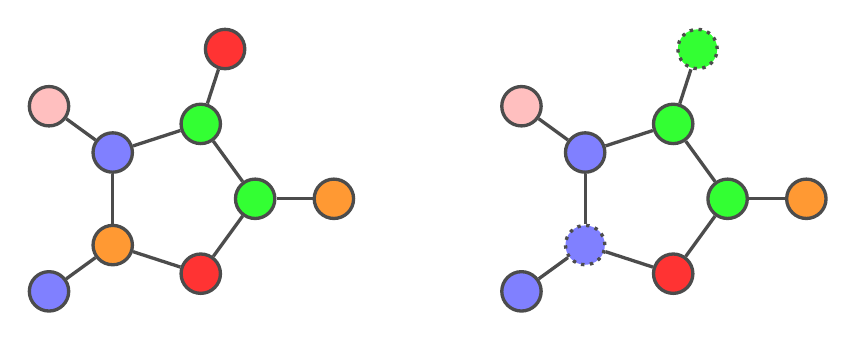
\begin{tikzpicture}
        \foreach[count=\i] \a \d \c in {
            0/1/1,72/1/1,144/1/2,216/1/3,288/1/4%
            ,0/2/3,72/2/4,144/2/5,216/2/2%
        }{
            \node[c\c](\i) at(\a:\d){};
        }

        \foreach \u \v in {
            1/2,2/3,3/4,4/5,5/1%
            ,4/9,1/6,2/7,3/8%
        }{
            \draw (\u) -- (\v);
        }

        \begin{scope}[xshift=6cm]
            \foreach[count=\i] \a \d \c in {
                0/1/1,72/1/1,144/1/2,216/1/2d,288/1/4%
                ,0/2/3,72/2/1d,144/2/5,216/2/2%
            }{
                \node[c\c](\i) at(\a:\d){};
            }
    
            \foreach \u \v in {
                1/2,2/3,3/4,4/5,5/1%
                ,4/9,1/6,2/7,3/8%
            }{
                \draw (\u) -- (\v);
            }
        \end{scope}
        
    \end{tikzpicture}
    \end{center}
\end{frame}
\begin{frame}{Previous/\alert{Our} Work (non exhaustive)}
    \begin{figure}
    \centering
    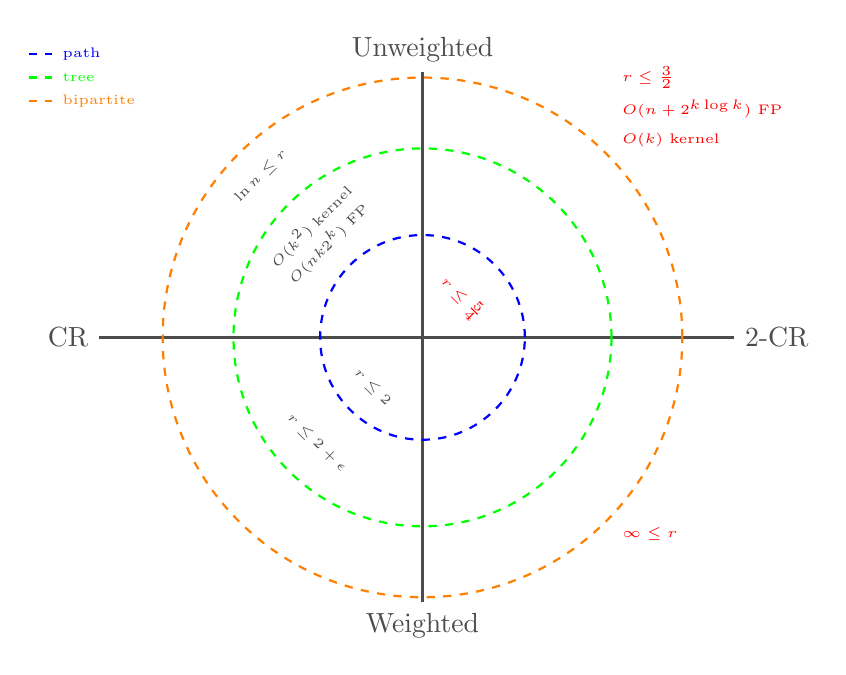
\begin{tikzpicture}[every node/.style={draw=none}]
    
    \node(cr) at(-4.5,0) {CR};
    \node(2cr) at(4.5,0) {2-CR};
    
    \node(weighted) at(0,-3.66) {Weighted};
    \node(unweighted) at(0,3.66) {Unweighted};
    
    \draw[] (cr) -- (2cr);
    \draw[] (weighted) -- (unweighted);
    
    \begin{scope}[thick, dashed]
    
    \draw[blue]	(-5,3.6) -- +(0.3,0) node[right]{\tiny path};
    \draw[green]	(-5,3.3) -- +(0.3,0) node[right]{\tiny tree};
    \draw[orange]	(-5,3) -- +(0.3,0) node[right]{\tiny bipartite};
    
    \draw[blue] (0,0) circle(1.3cm);
    \draw[green] (0,0) circle(2.4cm);
    \draw[orange] (0,0) circle(3.3cm);
    \end{scope}
    
    \begin{scope}[every node/.style={rotate=-45}]
    \node at(225:.9){\tiny$r \leq 2$};
    \node at(225:1.9){\tiny$r \leq 2 + \epsilon$};
    \end{scope}
    
    \begin{scope}[every node/.style={rotate=45}]
    \node at(135:1.7){\tiny $O(n k 2^{k})$ FP};
    \node at(135:2){\tiny $O(k^2)$ kernel};
    \node at(135:2.9){\tiny$\ln n \leq r$};
    \end{scope}
    
    \node[red, rotate=-45] at(45:.7){\tiny $r \leq \frac{5}{4}$};
    \begin{scope}[anchor=west]
    \node[red] at(2.4,2.5){\tiny $O(k)$ kernel};
    \node[red] at(2.4,2.9){\tiny $O(n + 2^{k\log k})$ FP};
    \node[red] at(2.4,3.3){\tiny $r \leq \frac{3}{2}$};
    \node[red] at(2.4,-2.5){\tiny $\infty \leq r$};
    \end{scope}
    
    \begin{scope}[]
    \end{scope}
    
    \end{tikzpicture}
    \end{figure}
    \end{frame}
\begin{frame}{Algorithm}
\begin{center}
    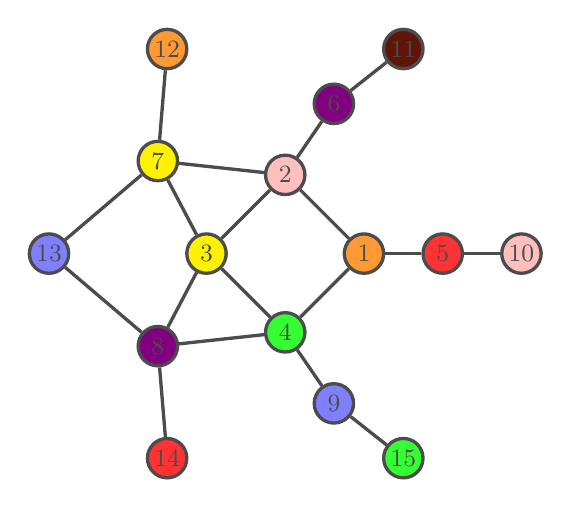
\begin{tikzpicture}[]
        \node[c3, on=<6->{c5}](1) at(0:1) {1};
        \node[c5](2) at(90:1) {2};
        \node[c7](3) at(180:1) {3};
        \node[c1](4) at(270:1) {4};
        \node[c4, on=<6->{c5}](5) at(0:2) {5};
        \node[c6, on=<8->{fill=none}](6) at(72:2) {6};
        \node[c7](7) at(144:2) {7};
        \node[c6](8) at(216:2) {8};
        \node[c2, on=<4->{c1}](9) at(288:2) {9};
        \node[c5](10) at(0:3) {10};
        \node[c8](11) at(60:3) {11};
        \node[c3](12) at(120:3) {12};
        \node[c2](13) at(180:3) {13};
        \node[c4](14) at(240:3) {14};
        \node[c1](15) at(300:3) {15};

        \draw (1) -- (2);
        \draw[on=<5->{blur}] (1) -- (4);
        \draw (1) -- (5);
        
        \draw[on=<3->{blur}] (2) -- (3);
        \draw[on=<7->{blur}] (2) -- (6);
        \draw[on=<3->{blur}] (2) -- (7);
        
        \draw[on=<3->{blur}] (3) -- (4);
        \draw (3) -- (7);
        \draw[on=<3->{blur}] (3) -- (8);
        
        \draw[on=<5->{blur}] (4) -- (8);
        \draw (4) -- (9);
        
        \draw (5) -- (10);
        
        \draw[on=<2->{blur}] (6) -- (11);
        
        \draw[on=<3->{blur}] (7) -- (12);
        \draw[on=<3->{blur}] (7) -- (13);
        
        \draw (8) -- (13);
        \draw (8) -- (14);
        
        \draw (9) -- (15);
    \end{tikzpicture}
\end{center}
\end{frame}

\begin{frame}{Service Chain Placement in SDNs}
\centering
\begin{tikzpicture}[every node/.append style={draw=none}, -, thick]

    % ANIMATIONS
    
    \def\timeDeploy{2-} 
    \def\timeCpu{3} 
    \def\timeBw{4} 
    \def\timeLat{5} 
    \def\timeCost{6} 
    
    % TITLES
    \node at(0,2) {SDN};
    \node at(0,-4) {Service Chain};
    
    % SDN
    \begin{scope}[y=.6cm]
    
    \begin{scope}[on=<{\timeDeploy}>{blur}]
    \node(2) at(2,3) {\faServer};
    \node(3) at(3,-2) {\faServer};
    \node(6) at(6,3) {\faServer};
    \end{scope}
    
    \node(0) at(0,1) {\Huge \faCloud};
    \node(4) at(4,1.5) {\faServer};
    \node(7) at(6.5,-1) {\faServer};
    \node(9) at(9,1) {\Huge \faCloud};
    
    \node[on=<{\timeDeploy}>{orange}](1) at(1.5,1) {\faServer};
    \node[on=<{\timeDeploy}>{blue}](5) at(4.5,-1) {\faServer};
    \node[on=<{\timeDeploy}>{red}](8) at(7.5,1) {\faServer};
    
    \end{scope}
    % /SDN
    
    \begin{scope}[on=<{\timeDeploy}>{blur}]
    \draw (6) -- (8);
    \draw (1) -- (2);
    \draw (1) -- (3);
    \draw (2) -- (4);
    \draw (3) -- (4);
    \draw (3) -- (5);
    \draw (4) -- (6);
    \draw (5) -- (6);
    \draw (6) -- (7);
    \end{scope}
    
    \begin{scope}[on=<{\timeDeploy}>{->}]
    \draw (0) -- (1);
    \draw (1) -- (4) node[label above] {\only<{\timeBw}>{$\geq 80$\mb}};
    \draw (4) -- (5) node[label above] {\only<{\timeBw}>{$\geq 80$\mb}};
    \draw (5) -- (7) node[label below] {\only<{\timeBw}>{$\geq 40$\mb}};;
    \draw (7) -- (8) node[label below] {\only<{\timeBw}>{$\geq 40$\mb}};;
    \draw (8) -- (9);
    \end{scope}
    
    
    % SC
    \begin{scope}[
        xshift=1cm
        , yshift=-2.5cm
        , ->
        , every node/.append style={
            rectangle
            , minimum height=4mm
            % , draw
        }
    ]
    
    \node(s) at(-1, 0){\Huge \faCloud};
    
    \begin{scope}[on=<{\timeDeploy}>{every node/.append style={orange}}]
    \node(f1) at(1,0) {\faWrench};
    \node(f2) at(2,0) {\faFlash};
    \end{scope}
    
    \begin{scope}[on=<{\timeDeploy}>{every node/.append style={blue}}]
    \node(f3) at(3,.5) {\faGear};
    \node(f5) at(4,0) {\faFilter};
    \node(f6) at(5,0) {\faTint};
    \end{scope}
    
    \node[on=<{\timeDeploy}>{blur}](f4) at(3, -.5){\faGears};
    
    \begin{scope}[on=<{\timeDeploy}>{every node/.append style={red}}]
    \node(f7) at(6,0) {\faFlask};
    \end{scope}
    
    \node(t) at(8, 0){\Huge \faCloud};
    
    \begin{scope}[on=<{\timeDeploy}>{blur}]
    \draw (f2) -- (f4);
    \draw (f4) -- (f5);
    \end{scope}
    
    \draw (s) -- (f1);
    \draw (f1) -- (f2);
    \draw (f2) -- (f3) node[label above] {\only<{\timeBw}>{80\mb}};
    \draw (f3) -- (f5);
    \draw (f5) -- (f6);
    \draw (f6) -- (f7) node[label below] {\only<{\timeBw}>{40\mb}};
    \draw (f7) -- (t);
    \end{scope}
    % /SC
    
    % CPU
    \only<{\timeCpu}>{
    \begin{scope}[every node/.style={label}]
    \node[below=0 of 1]{$\geq 8$\cpu};
    \node[below=0 of 5]{$\geq 12$\cpu};
    \node[above=0 of 8]{$\geq 5$\cpu};
    
    \node[above=0 of f1]{3\cpu};
    \node[above=0 of f2]{5\cpu};
    
    \node[below=0 of f3]{2\cpu};
    \node[below=0 of f5]{4\cpu};
    \node[below=0 of f6]{6\cpu};
    
    \node[above=0 of f7]{5\cpu};
    \end{scope}
    }
    % /CPU
    
    % LAT
    \onslide<{\timeLat}>{
    \begin{scope}[dashed, ->]
    \draw (0) to[bend left] node[label above] {$\leq 90$\ms} (9);
    \draw (s) to[bend right] node[label below] {90\ms} (t);
    \end{scope}
    }
    % /LAT
    
    \only<{\timeCost}>{
    \begin{scope}[every node/.style={label}]
    \node[below=0 of 1]{7\$};
    \node[below=0 of 5]{4\$};
    \node[above=0 of 8]{9\$};
    \end{scope}
    }
    
    \end{tikzpicture}
    
\end{frame}
\begin{frame}{Service Chain Placement in SDNs}
    Minimize Placement Cost

    s.t.
    \begin{itemize}
        \item CPU
        \item Bandwidth
        \item Latency
    \end{itemize}
\end{frame}
\begin{frame}{Our Results}

\begin{itemize}[<+>]
  \item NP-hardness in many cases 
\end{itemize}

\vspace{5mm}
\onslide<+->
 
\def\arraystretch{1.5}
\begin{tabular}{c | c | l}
SDN	& Costs	& Our Result
\\
\hline
\onslide<+->{%
\color{red} DAG	& \color{red}Integral, Polynomial 		& \color{green}Optimal
}
\onslide<+->{
\\
\color{red}DAG	& \color{green}Any				& \color{green}FPTAS - ($1+\varepsilon$)-apx
}
\onslide<+->{
\\
\color{green}Any	& \color{green}Any			& \color{orange}FPTAS - ($1+\varepsilon$)-apx\onslide<+>{\footnote{%
\onslide<.>{running time depends on SDN's typology}}} }

\end{tabular}
\vspace{2cm}
\end{frame}

\input{frame-cm-problem}
\input{frame-cm-problem-cont}
\input{frame-cm-prev}

% \input{frame-budgeted-coverage-lemma}
% \input{frame-budgeted-coverage-lemma-example}
% \input{frame-modified-greedy}
\begin{frame}{Submodular Maximization with a Knapsack Constraint}
    \begin{itemize}
        \item a ground set $U$
        \item a cost function $c:U \to \mathbb{R}$
        \item a budget $B$
        \item a monotone\footnote{
                $\forall A \subseteq B \subseteq U: f(B) \geq f(A)$
            }, submodular\footnote{
                $\forall A, B \subseteq U: f(A) + f(B) \geq f(A \cup B) + f(A \cap B)$
            } function, $f:2^U \to \mathbb{R}$
        \item find $S$ that maximizes $f$ s.t. $c(S) \leq B$
    \end{itemize}
\end{frame}


\input{frame-submodular-prev}
\input{frame-submodular-greedy}
\begin{frame}{Lemma}
    \begin{Lemma}
        Let $B \subseteq U$ and let $A \subseteq U$ chosen greedily such that $A \cap B = \emptyset$ then $f(A) \geq (1 - e^{-\frac{|A|}{|B|}})f(B)$
    \end{Lemma}
\end{frame}
\begin{frame}{Modified Greedy}
    $$
    \argmax_{\mathclap{S \in \{G, \argmax_{a \in U}f(a)\}}}f(S)
    $$
\end{frame}
\begin{frame}{Correct Proof}
    Assume that $f(A) = (1 - e^{-\frac{1}{2} + \delta})$
    \begin{center}
        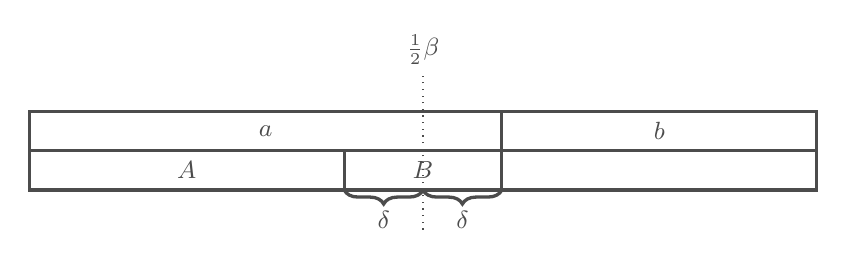
\begin{tikzpicture}
            \draw (0,0)  rectangle (10, 1);
            \draw[thin, dotted] (5, -.5) -- (5, 1.5) node[above, draw=none]{$\frac{1}{2}\beta$};
            \draw[] (0,0) rectangle (4, .5) node[midway, draw=none]{$A$};
            \draw (0, .5) rectangle (6, 1) node[midway, draw=none]{$a$};
            \draw[decorate,decoration={brace,amplitude=5pt, mirror}]
                    (4,0) -- (5,0) node[midway, below=1mm, draw=none]{$\delta$};
            \draw[] (6, .5) rectangle (10, 1) node[draw=none, midway]{$b$};
            \draw[decorate,decoration={brace,amplitude=5pt, mirror}]
                    (5,0) -- (6,0) node[midway, below=1mm, draw=none]{$\delta$};
            \draw (4, 0) rectangle (6, .5) node[draw=none, midway]{$B$};
        \end{tikzpicture}
    \end{center}
    $$
    \begin{array}{ll}
        f(B|A) & \geq (1 - e^{\frac{2\delta}{\frac{1}{2} - \delta}})f(O \setminus A \setminus a)
        \\
        & \geq (1 - e^{\frac{2\delta}{\frac{1}{2} - \delta}})(f(O) - f(A) - f(a))
        \\
        & \vdots
        \\
        f(A \cup B) & \geq f(A) + f(B|A) \geq \dots \geq (1 + e^{-\frac{1}{2}})f(O)
    \end{array}
    $$
\end{frame}
\begin{frame}{Modified$^2$ Greedy}
    $$
    \argmax_{\mathclap{S \in \{G, \argmax_{\{a,b\} \in U}f(\{a, b\})\}}}f(S)
    $$

    \pause
    \begin{theorem}
        $(1 - e^{-(\frac{1}{2} + 0.104)})$-approximation.
    \end{theorem}
\end{frame}
\begin{frame}{Boosting Framework}
    \begin{Theorem}
        For every $\alpha < \beta < \frac{1}{2}$, given an $\alpha$-approximation 
        algorithm with running time $O(n^2)$ we can produce a $\beta$-approximation algorithm 
        with running time $O(n^2)$.
    \end{Theorem}
\end{frame}
\begin{frame}{Boosting Framework - Intuition}
        \begin{itemize}[<+(1)>]
            \item Let $\gamma = c(a)$ for some $a \in O$
            \item Let $b = \displaystyle{\argmax_{\mathclap{e \in U : c(e) \leq \gamma}} f(e)}$
            \item Choose $b$ and recurse on $U \setminus \{a, b\}, O \setminus a, f_b$
        \end{itemize}
\end{frame}
\begin{frame}{More Intuition}
    \begin{itemize}[<+(1)>]
        \item Let $O_{\frac{1}{3}} = \{e \in O : c(e) \leq \frac{1}{3}\}$    
        \item If $O = O_{\frac{1}{3}}$ then $f(G) \geq (1 - e^{-\frac{2}{3}})$
        \item If $|O \setminus O_{\frac{1}{3}}| = 2$ then $f(G) \geq (1 - e^{-2})f(O_{\frac{1}{3}}) \approx 0.86f(O_{\frac{1}{3}})$
    \end{itemize}
\end{frame}
\input{frame-submodular-alg}
% \input{frame-bucket-analysis}
% \begin{frame}{Conclusion}
    \begin{itemize}[<+(1)>]
        \item A tradeoff between speed and approximation
        \item Boosting framework might be of independent interest
    \end{itemize}
\end{frame}

% \input{sep-carpool-revisited}
% \input{frame-carpool-revisited}
% \input{frame-submodular-cont}
% \input{frame-submodular}
% \input{frame-spectrum}
% \input{frame-prev}

% \input{frame-thank-you}

\end{document}